\documentclass[a4paper,12pt]{article}
\usepackage[margin=1in]{geometry}
\usepackage{tikz}
\usepackage{listings}

\usetikzlibrary{shapes, arrows, positioning, calc}
\setlength{\parindent}{0pt}

\begin{document}

\title{Lista 1}
\author{Eduardo Henrique Basilio de Carvalho}
\date{\today}

\maketitle

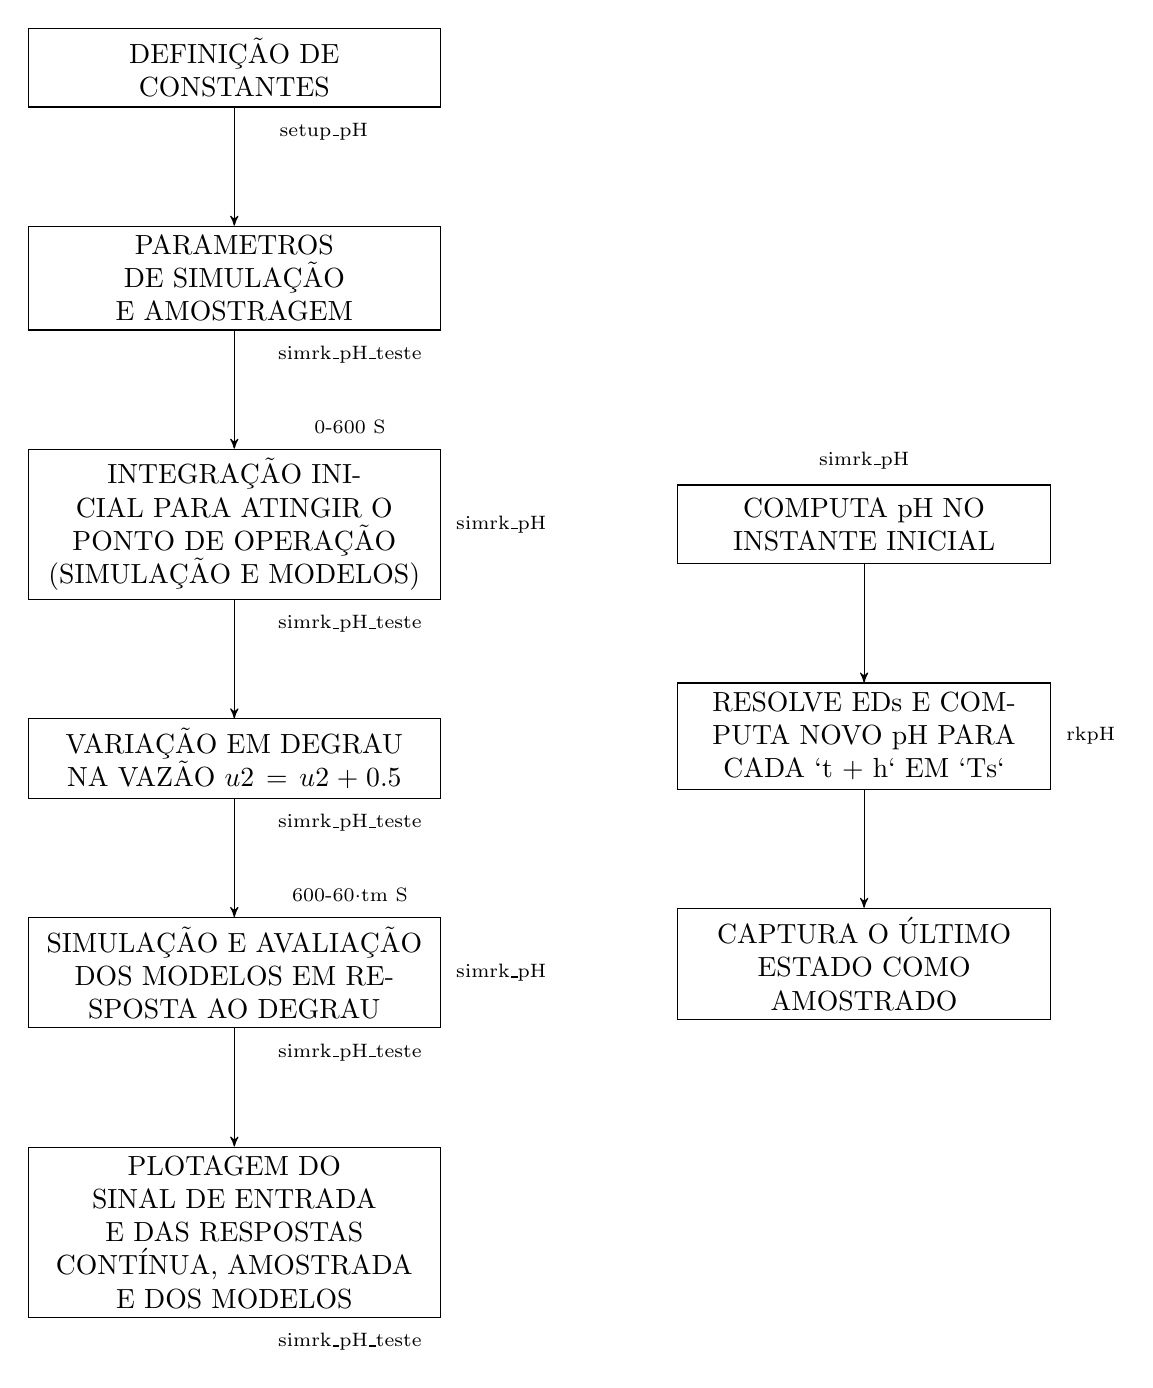
\begin{tikzpicture}[
  node distance=1.5cm and 1cm,
  block/.style={rectangle, draw, text width=5cm, minimum height=1cm, align=center},
  subblock/.style={rectangle, draw, text width=4.5cm, minimum height=1cm, align=center},
  func/.style={rectangle, draw, text width=3cm, minimum height=0.7cm, align=left,font=\scriptsize},
  annbelow/.style={font=\scriptsize, below=2pt},
  annabove/.style={font=\scriptsize, above=2pt},
  annside/.style={font=\scriptsize, right=2pt},
  arrow/.style={->, >=stealth'},
]

% Main Flow
\node[block] (setup) {DEFINIÇÃO DE CONSTANTES};
\node[block, below=of setup] (param) {PARAMETROS DE SIMULAÇÃO E AMOSTRAGEM};
\node[block, below=of param] (integracao) {INTEGRAÇÃO INICIAL PARA ATINGIR O PONTO DE OPERAÇÃO (SIMULAÇÃO E MODELOS)};
\node[block, below=of integracao] (variacao) {VARIAÇÃO EM DEGRAU NA VAZÃO \( u2 = u2 + 0.5 \)};
\node[block, below=of variacao] (simulacao) {SIMULAÇÃO E AVALIAÇÃO DOS MODELOS EM RESPOSTA AO DEGRAU};
\node[block, below=of simulacao] (plotagem) {PLOTAGEM DO SINAL DE ENTRADA E DAS RESPOSTAS CONTÍNUA, AMOSTRADA E DOS MODELOS};

% Annotations
\node[annbelow] at (setup.south) {\ \ \ \ \ \ \ \ \ \ \ \ \ \ \ \ \ \ \ \ \ \ \ \ setup\_pH};
\node[annbelow] at (param.south) {\ \ \ \ \ \ \ \ \ \ \ \ \ \ \ \ \ \ \ \ \ \ \ \ \ \ \ \ \ \ \ simrk\_pH\_teste};
\node[annbelow] at (integracao.south) {\ \ \ \ \ \ \ \ \ \ \ \ \ \ \ \ \ \ \ \ \ \ \ \ \ \ \ \ \ \ \ simrk\_pH\_teste};
\node[annabove] at (integracao.north) {\ \ \ \ \ \ \ \ \ \ \ \ \ \ \ \ \ \ \ \ \ \ \ \ \ \ \ \ \ \ \ 0-600 S};
\node[annside] at (integracao.east) {simrk\_pH};
\node[annbelow] at (variacao.south) {\ \ \ \ \ \ \ \ \ \ \ \ \ \ \ \ \ \ \ \ \ \ \ \ \ \ \ \ \ \ \ simrk\_pH\_teste};
\node[annbelow] at (simulacao.south) {\ \ \ \ \ \ \ \ \ \ \ \ \ \ \ \ \ \ \ \ \ \ \ \ \ \ \ \ \ \ \ simrk\_pH\_teste};
\node[annabove] at (simulacao.north) {\ \ \ \ \ \ \ \ \ \ \ \ \ \ \ \ \ \ \ \ \ \ \ \ \ \ \ \ \ \ \ 600-60\(\cdot\)tm S};
\node[annside] at (simulacao.east) {simrk\_pH};
\node[annbelow] at (plotagem.south) {\ \ \ \ \ \ \ \ \ \ \ \ \ \ \ \ \ \ \ \ \ \ \ \ \ \ \ \ \ \ \ simrk\_pH\_teste};

% simrk_pH Subprocess
\node[subblock, right=3cm of integracao] (comp) {COMPUTA pH NO INSTANTE INICIAL};
\node[subblock, below=of comp] (resolve) {RESOLVE EDs E COMPUTA NOVO pH PARA CADA `t + h` EM `Ts`};
\node[subblock, below=of resolve] (captura) {CAPTURA O ÚLTIMO ESTADO COMO AMOSTRADO};

\node[annabove] at (comp.north) {simrk\_pH};
\node[annside] at (resolve.east) {rkpH};

% Connections
\draw[arrow] (setup) -- (param);
\draw[arrow] (param) -- (integracao);
\draw[arrow] (integracao) -- (variacao);
\draw[arrow] (variacao) -- (simulacao);
\draw[arrow] (simulacao) -- (plotagem);

\draw[arrow] (comp) -- (resolve);
\draw[arrow] (resolve) -- (captura);

\end{tikzpicture}

\texttt{simrk\_pH}: simula a planta por um tempo de amostragem. recebe os parametros relevantes, o instante inicial da iteração e o estado do sistema neste instante

\texttt{rkpH}: computa o novo estado usando o método de Runge-Kutta de 4ª ordem; chama \texttt{dvpH}

\texttt{dvpH}: computa as equações diferenciais a partir das entradas e do estado atual

A resposta dos modelos depende do intervalo de amostragem. Quanto menor, mais rápida a resposta.

Integração numérica é o calculo da área sob uma curva por abordagens geométricas e aritméticas, em oposição à integração analítica, que usa regras algébricas.

Em \texttt{simrk\_ph\_CD}, o controlador implementado é proporcional:
\begin{lstlisting}[language=matlab]
  m(k-1) = K*e(k-1);
  u2(k-1) = Q3(k-1)+m(k-1);
\end{lstlisting}

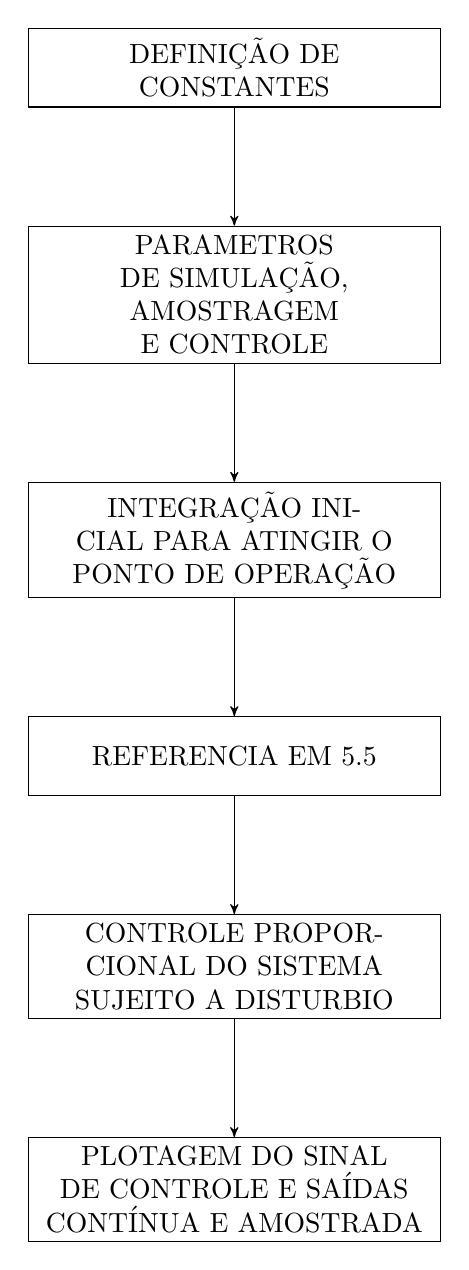
\begin{tikzpicture}[
  node distance=1.5cm and 1cm,
  block/.style={rectangle, draw, text width=5cm, minimum height=1cm, align=center},
  func/.style={rectangle, draw, text width=3cm, minimum height=0.7cm, align=left, font=\scriptsize},
  annside/.style={font=\scriptsize, right=2pt},
  arrow/.style={->, >=stealth'}
]

% Main Flow
\node[block] (setup) {DEFINIÇÃO DE CONSTANTES};
\node[block, below=of setup] (param) {PARAMETROS DE SIMULAÇÃO, AMOSTRAGEM E CONTROLE};
\node[block, below=of param] (integracao) {INTEGRAÇÃO INICIAL PARA ATINGIR O PONTO DE OPERAÇÃO};
\node[block, below=of integracao] (variacao) {REFERENCIA EM 5.5};
\node[block, below=of variacao] (simulacao) {CONTROLE PROPORCIONAL DO SISTEMA SUJEITO A DISTURBIO};
\node[block, below=of simulacao] (plotagem) {PLOTAGEM DO SINAL DE CONTROLE E SAÍDAS CONTÍNUA E AMOSTRADA};

% Connections
\draw[arrow] (setup) -- (param);
\draw[arrow] (param) -- (integracao);
\draw[arrow] (integracao) -- (variacao);
\draw[arrow] (variacao) -- (simulacao);
\draw[arrow] (simulacao) -- (plotagem);

\end{tikzpicture}

O trecho de controle é atingido com mesmo período que o trecho de simulação contínua. Entretanto, como o erro é computado a partir da saída amostrada, este é atualizado com o período de amostragem. Dado que o controle proporcional depende apenas do erro instantâneo, não do erro acumulado ou da tendencia de sua variação, o estado de controle também tem o período da amostragem.

\end{document}